\documentclass[10]{article}
\usepackage{preamble}

\title{Foundations of Discrete-Event Simulation \\ \footnotesize{Theoretical and practical aspects using the example of card games}}

\author{Pascal Crenzin}
\date{21.08.2020}

\begin{document}
	\maketitle
	\begin{abstract}
	This report introduces discrete-event simulations and classifies the purpose of discrete-event simulation based on its characteristics. Discrete-event simulations are stochastic, dynamic and based on discrete events. Every simulation is based on a model. A generic model of discrete-event simulation is the queuing of arriving events, followed by the processing of the events. Every event changes the system state. An application of using discrete-event simulation to analyze and balance card games is demonstrated with the example of \uno. The presented approach realizes the main components and the simulation paradigm in a custom implementation of a framework for the simulation of card games. The simulation of \uno\ analyzes the duration of \uno\ games depending on the presence of special cards, number of players and number of initial hand cards. The result is, that a \uno\ game takes normally 10 to 30 rounds to finish.
	\end{abstract}
	\newpage
	\tableofcontents
	\newpage
  %!TEX root=../report.tex

%grammarly checked

\section{Introduction}


Simulations are a problem-based discipline that allows for repeated testing of a hypothesis \cite{sokolowski2010modelingintro}. This statement covers two important aspects of simulations in general. The first key element in this statement is \textit{“problem-based”}. This means a simulation always addresses a question. The second key element is \textit{“repeated testing”}. This means a simulation is intended to run multiple times.


The field of simulations covers a wide range of applications.
Simulations, in particular, discrete-event simulations can be used to analyze the complex behavior of systems.
Examples are stock inventory monitoring, optimizing supply chains \cite{krenczyk2014production}, health care systems \cite{jacobson2006discrete, jun1999application} or games.

In order to simulate a real-world system, a model must be created. All observations are derived from the model. Understanding the foundations of how to build such models is the base for data-driven insights. It enables people to build a precise abstraction of reality, having a methodology to master complexity, understand required techniques and tools, and prove its validity by solid mathematical foundations \cite{sokolowski2010modelingintro}.

This report sets its focus on the simulation of board games, especially card games.

Board games are discussed by researchers in multiple branches of science like social science, computer science, mathematics, or psychology. Board games are either object of study or models for developing analogies \cite{gobet2004moves}. An example of an analogy is by Janssen who used the analysis of shredded card games to understand the evolution of institutional arrangements \cite{janssen2010evolution}.
If the board game becomes the object of research a simulation can be used to train a computer on how to play a game. A popular example is the development of AlphaGo \cite{silver2017mastering}. Another approach is to use simulations during the game design phase which is more challenging than gameplay. This can be done by tuning the game parameters or by modifying the rules \cite{hom2007automatic}.
To achieve the right balance of fun, time, or easiness of the game, parameters and rules must be chosen carefully. For example the number of cards at the beginning of a game or the number of jokers in the game. Using simulations makes it simple to collect quantitative data about little details that can have a huge impact on the game.

This report continues with the foundations of discrete-event simulation, followed by an example simulation of the card game \uno. Then, the design of \uno\ will be analyzed. After that I discuss the model of \uno\ and finally, I draw a conclusion.


%Simulations can play a role to understand player behavior.

% The large diversity of rules of shedding games show that this kind of game allows for tinkering of the rules and makes interesting variations of the same base game. Including or excluding a rule doubles the overall number of combinations. This means a game that is based on five rules could exist in 2^5 different variations.



%Board games are an interesting field for simulations because they consist of a clear set of rules and discrete events.



  %!TEX root=../report.tex

\section{Foundations}


Simulations are a \textit{problem-based discipline that allows for repeated testing of a hypothesis.} \cite{sokolowski2010modelingintro} This statement covers two important aspects of simulations in general. The first key element in this statement is \textit{“problem-based”}. This means a simulation always addresses a question. The second key element is \textit{“repeated testing”}. This means a simulation is intended to run multiple times.

The general approach to simulate something is to build a model as an abstraction of a system in the real world and then modify and observe the model according to the hypothesis that needs to be tested. The last step is to draw a conclusion out of the observations.

\subsection{Terminology}

System and model are widely used. To clarify their meaning in this report I explain their meaning in the context of simulations.

\subsubsection{System}

A model is intended to represent a system in the real world. Therefore the abstract term \textit{system} must be defined. In the scope of this report, a system is a collection of different elements that influence the simulation. This includes among other people, hardware, software, institutions, documents, and environmental factors. A system can be physically present in the real world, but it could also be a plan or concept for something that does not exist.

\subsection{Event}
\note{Something that my occur}

\subsubsection{Model}

The concept \textit{model} is a physical, mathematical, or otherwise logical
representation of a system. Models serve as representations of events and things. The events can be real, e.g. from an observation of the real world, or contrived. A model represents a system.
While a system could be dangerous to observe or even don't exist, a model could be used to study the evolution of a system. When investigating a system, a quantitative assessment is derived. This may include how the system performs with various inputs and in different environments.
Different scenarios (occurrence of specific events) can be investigated.  It is important to get a quantitative evaluation of the performance of the system. The performance could cover multiple aspects, which depend on the purpose of the model.
A model exists at three levels of abstraction: conceptual, specification, and computational. \cite[chapter 1]{leemis2006discrete} A conceptual model abstracts the general concept while a specification model contains concrete information. A computational model refers to an implemented program of a model, which means that the computational model is nothing else than a simulation. In this report computational model and simulation are equivalent. The classifications for simulations are also classifications of models.

In the following, I will go into more detail regarding different types of simulations, followed by a detailed explanation of discrete-event simulation, and lastly, introduce the cycle of modeling \& simulation.


\subsection{Classification of Simulations}


Simulations in general can be classified depending on multiple aspects. In this section, I will introduce a few approaches to classify simulations.

\subsubsection{Static \& Dynamic}

A system model is static or dynamic. A static model is one in which time
is not a significant variable. A dynamic model evolves over time. \cite{leemis2006discrete} \note{(chapter 1)}

Static models can answer the question of how much money gets distributed if \textit{N} people play the lottery next week. The result is completely independent of the timing of the players.
To solve such questions, there is the Monte Carlo simulation, that relies on repeated random sampling to obtain numerical results. Another use case for Mone-Carlo simulations is finding the area under a curve. \cite{ohriner1971finding}

If the system evolves over time it is a so-called dynamic model. A dynamic model would emerge if the lottery example gets extended by players that play week for week. Their spendings on the lottery could depend on their last result.


\subsubsection{Continuous \& Discrete}

A dynamic system model is continuous or discrete. Continuous simulations are based on a continuous function of time. Examples of continuous simulations can be found in classical mechanics. Examples are oscillating pendulums or a block sliding on an inclined plane. In each of these cases, the motion is characterized by one or more differential equations that model the continuous-time evolution of the system.
In contrast, discrete simulations are based on events that occur at discrete points in time. Only events can lead to a change in the system. Examples are inventory systems or board games.
An inventory system changes its state every time a new order arrives or new products arrive. These changes are not continuous, but they occur at a certain point in time.
The next section focuses on discrete-event simulation in more detail.

\begin{figure}[h!]
 \caption{Chosing the right simulation paradigm depending on the model requirements (adopted from \cite[page 3]{leemis2006discrete})}
 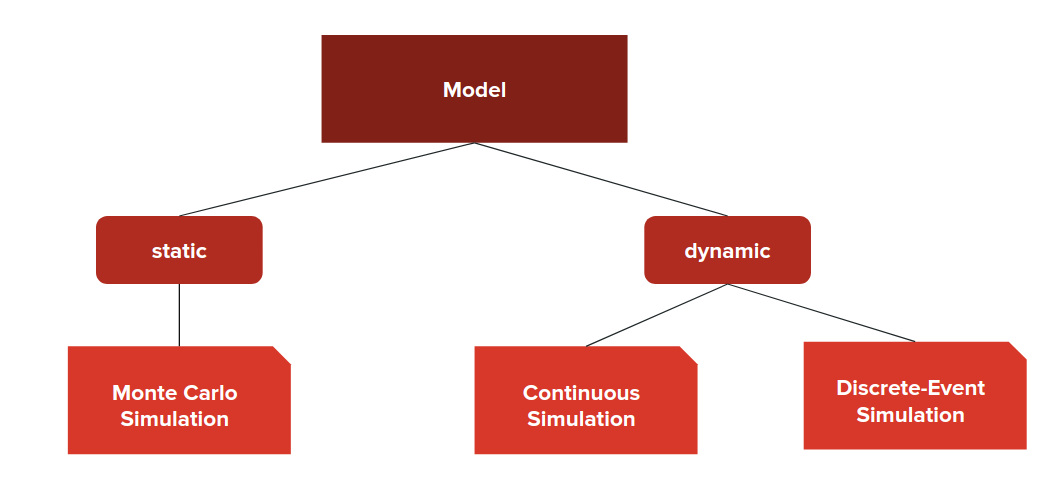
\includegraphics[width=0.9\textwidth]{static-dynamic-classification}
\end{figure}


\subsubsection{Fidelity, Resolution \& Scale}

There are three primary attributes that can be mapped to models or simulations.
These are fidelity, resolution, and scale. \cite{sokolowski2010modelingintro}

\textbf{Fidelity} indicates how close a simulation matches reality. A model that closely behaves like a real system has high fidelity. High fidelity means that every aspect of the system must be covered. Normally models aim to describe only the parts that are necessary for the initial hypothesis. Aiming for a high fidelity would mean a great effort. It should only be done if the hypothesis requires a high fidelity of the simulation.


\textbf{Resolution} describes the level of details. The more detail included in the simulation, the
higher the resolution. To illustrate this, a model of a plantation could be broken down into models of all single plants. Modeling all plants would achieve a higher resolution. The target resolution depends on the intention of the model. Referring to the plantation example, a model that should describe harvesting around the globe, would better use a low resolution, namely models of plantations, while a model to optimize the crop would need a higher resolution.

\textbf{Scale} indicates the overall size of the simulation. A larger system has a higher scale. The scale is a fairly subjective metric. It always depends on the relations. One example is simulating a fabric compared to simulating a single device in a production line.


\subsubsection{Games, Simulation Games \& Simulators}


Nearly every system can be simulated. In this report, I would like to have a deeper look into the field of games. Games play a popular role in the entertainment industry. There is a wide range of games that aim to simulate a system in an interactive way. These can be distinguished whether they aim for fun or for training.
Games, simulation games, and simulators can be distinguished based on various characteristics. \cite{narayanasamy2006distinguishing} In this scope \textit{games} mainly refers to computer games. But the characteristics also apply for board games.
All (computer) games have a simulation part somehow, but one characteristic is that simulation games do not always involve a specific goal-oriented activity within the context of the game. Games and simulation games aim for fun and entertainment. They provide challenges and have typical game patterns. The world can be imaginative or fictitious.
Simulators are designed for training. Training simulators only provide a real-world environment. They aim for skill-development rather than fun. Challenges in training simulators are challenges with equivalents in the real-world.



\subsection{Discrete-Event Simulation}

There are certain characteristics that define a discrete event simulation.
First of all, there must be a stochastic component. This means the state of our model depends on probabilities. At least one variable that defines the current state of the system must be random.
Secondly, the model is dynamic. This means, there is a change over time.
Thirdly, the changes of the model depend on discrete-events. These discrete-events can occur randomly at discrete time instances.


\begin{figure}[h!]
 \caption{Visualization of a discrete-event simulation system}
 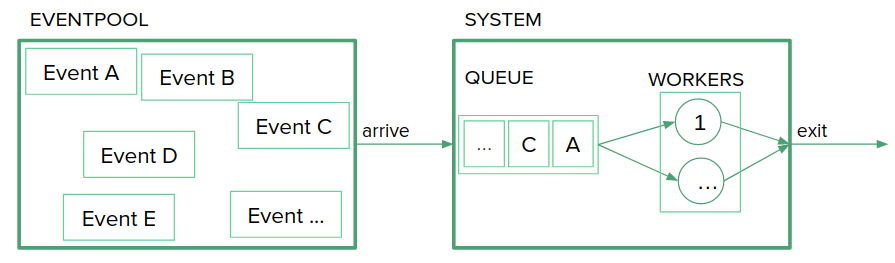
\includegraphics[width=0.9\textwidth]{queue-model}
\end{figure}

To visualize a discrete-event simulation, it can be seen as a queuing system. There are certain events that can occur and a system contains queue and workers that handle the events.
Depending on the scenario events are also called jobs or customers. Workers also have synonyms like server. The queue is sometimes renamed to \textit{event list} or \textit{calendar}. And the system is also called \textit{service node} in other literature.
Events arrive at the system at random points in time and each event could take a different amount of time to get processed by a worker before the event it can exit the system. The systems operate as follows: If a new event arrives, it will be moved into the queue. If the queue is not empty and at least one worker is not busy, one event is taken from the queue and gets processed.

From this behavior, two important terms regarding the timing can be derived.
Delay. The delay is the time that an event remains in the queue. the delay is greater or equals zero.
Wait. The wait for an event is the duration between arrival and exit. In other words, the wait is the delay plus the processing time of the worker.

Reducing delay and wait is a common optimization goal that discrete-event simulation can be used for. This could be achieved by adding more workers or changing the way how events are selected from the queue. A common technique is FIFO (first in, first out) that always takes the event with the greatest delay. Other techniques try to optimize the delay by prioritizing events with a small processing time (also known as \textit{shortest job first}).

\subsubsection{Components}
\label{des:components}

There are some main components that a discrete event simulation requires.

The System State. This captures all variables that characterize the simulation.

The Simulation Clock. This is a tool that tracks the elapsed time. Different approaches to increment the simulation clock are explained in \hyperref[des:timeadvance]{\textit{Time-Advance Mechanism}}.

Next - Event List. This is a queue for the upcoming events.

Statistical Counter or Accumulator. This is a tool that records the evolution of the system state.
%
%The initialization program is the setup method of the game class.
%
%
%The event subprogram is in the simulate function of the game class. In pseudo code the simulate functions runs in a loop till the game is finished. And we call the player.play function that modifies the current game state. This function contains all the logic to play the game. In my implementation it’s pick a card with the same color or same number otherwise take a card from the draw pile.
%
%The event subprogram is in the simulate function of the game class. In pseudo code the simulate functions runs in a loop till the game is finished. And we call the player.play function that modifies the current game state. This function contains all the logic to play the game. In my implementation it’s pick a card with the same color or same number otherwise take a card from the draw pile
%.

%
%(5) Initialization Subprogram. A protocol utilized in the initialization of
%the simulation, usually setting the start time to zero.
%(6) Timing Subprogram. A protocol that, drawing from a next - event list,
%sets the next event and progresses the simulation clock to the moment
%when an event is to happen.
%(7) Event Subprogram. A protocol that launches a routine that updates
%the state of the system with the occurrence of each event.
%(8) Library Subprogram. A protocol used to produce random observa-
%tions drawn generally from predetermined probability distributions.
%(9) Report Generator. A tool that calculates and reports statistics that
%describe the performance of the system.
%(10) Main Program. A routine that coordinates the concert of subordinate
%routines, executing these in the correct sequence. It initializes the
%timing subprogram that determines the subsequent event, passes
%control to the related event subprogram, and updates the system state.
%This routine verifi es for termination and triggers the report generator
%once the simulation ends.
%


\subsubsection{Trace-Driven Discrete-Event Simulation}

The events in a discrete-event simulation can be generated or prerecorded. If the simulation relies on prerecorded data, it is a so-called trace-driven discrete-event simulation.
By definition, a trace-driven simulation relies on input data from an external source to generate realistic events. \cite{leemis2006discrete} The advantage of trace-driven discrete-event simulations is that no data needs to be generated and the data source reveals realistic data. On the other hand, the reliance on external data limits the capabilities to simulate new scenarios. A common question is "What if \textit{X}" happens. And if \textit{X} not part of the recorded data it is not possible to find out.


\subsubsection{Next-Event Simulation}
\label{des:nextevent}

The concept of next-event simulation extends the basic concept of discrete-event simulations. To construct a next-event simulation model, all events must be assignable to an event type. An algorithm decides how the system state changes depending on these event types.
\cite[chapter 5]{leemis2006discrete}
The algorithm for a next-event simulation is based on four steps.
\textbf{Initialization.} In this The simulation clock is initialized (usually to zero) and the first events get queued.
\textbf{Processing the current event.} The queue is scanned to determine the next event. Then the event gets processed the event and the simulation clock advances.
\textbf{Schedule new events}. New events (if any) that may be spawned by the current event are placed in the queue.
\textbf{Terminate}. The process of advancing the simulation clock and processing events and scheduling new events continues until some terminal condition is satisfied. The terminal condition can be a specific event that only occurs once. Another terminal condition could be reaching a certain time on the simulation clock.


\subsubsection{Time-Advance Mechanism}
\label{des:timeadvance}

The progress of time in a simulation is a very essential aspect. In discrete-event simulations, there are two well-known approaches: Fixed-increment advance and next-event time advance.
The fixed-increment advance initializes at time zero and advances at fixed time increments. The disadvantage is that events occur not in sync with the increments. This means the arrival time and exit time is probably not exact. Another characteristic of the fixed-increment advance is that the size of the time increment is subjective. But choosing the increment interval has implications for the performance measures of the system. Large increments lead to imprecise timing of the events, while small increments could lead to a situation where no changes happen for many increments.
In contrast, the next-event time-advance approach is more versatile. It initializes the simulation clock at zero and then progresses to the next upcoming event. The incrementation step is not fixed, but always in sync with the arrivals and exits of all events. This solves the disadvantages of the fixed-increment advance.



% \note{Using Queues is a useful concept since we have queues everywhere in the real world. For example, if you order at an online shop your delivery gets processed at many    If you travel, you have to wait for your bus or your plane.}


\subsection{Modelling \& Simulation Cycle}

\begin{figure}[h!]
 \caption{Process of generating and evaluating simulations (adopted from \cite[page \note{X}]{sokolowski2010modeling})}
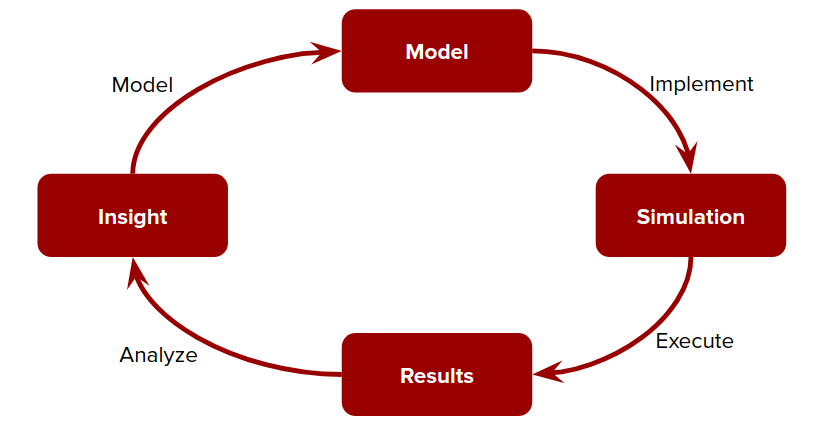
\includegraphics[width=0.9\textwidth]{simulation-modelling-cycle}
\end{figure}

Simulations are based on models and simulations are designed to answer a hypothesis. This means simulations must also be understood as a piece a larger process.
%The process of modeling and simulation is proposed by \note{Name}.
It starts with modeling. Modeling includes theories, information, algorithms of the topic. A decision must be taken which type of model and with paradigms are used. A supporting tool for that is the decision tree in \note{figure X}.
The result of the first phase is a model. The model gets implemented in the next step. There is dedicated software for simulation purposes. \cite{wiki:deslist} The result of this step is an executable program that implements the model.
During the execution phase, the simulation program generates data. For the execution, the processing environment must be taken into account. Complex simulations may need more computation power than a normal home computer could provide.
The output data must be transformed to get the desired performance insights.
If the model contains variability and uncertainty, then techniques from probability
and statistics will likely be required for the analysis. All further analysis must happen regarding the initial hypothesis. A model must be verified and validated. This means to check whether the model was built correctly and whether the model is appropriate compared to the real world.
 It is very likely that the results reveal that the model must be adjusted or extended. This means to reiterate through this cycle. It is a good practice to repeat the cycle as often as needed.

I will go through this cycle with an example of a discrete-event simulation use case in the next chapter.



  	%!TEX root=../report.tex

\section{Example: Model Card Games as Discrete-Event Simulation}


I focus on card games as examples. The focus on card games is due to the wide range of different types of board games. Board games, in general, are too diverse in terms of materials (game board, cards, meeples) and rules. In contrast to that, most card games share the same game elements. To be even more specific, the implementation mainly addresses shedding games, like \textit{UNO}, \textit{The Great Dalmuti} and \textit{Phase 10} \cite{wiki:sheddinglist}. They have at least one discard pile, where all players contribute to. They have a hand for each player and optionally a shared or not shared open played cards. And optionally they have a draw pile. Cards consist of color or a symbol, a number, and maybe a special rule is attached to them.
The game rules of card games are that all players take their turn one after the other. There is no concurrency. This excludes some card games that aim for competing in reaction time, but this is not the scope of this implementation.

The decision to build a framework from scratch was derived from the specific conditions that card games have.
In the next section, I will explain my implementation, followed by a concrete implementation of the card game Uno.

The objective of the implementation is to build a framework that

\begin{itemize}
\item map all main components of discrete-event simulation to the context of card games
\item uses an object-oriented approach for intuitive readability
\item is generic enough to cover common card games
\item keeps the implementation effort low for new player behavior and new games
\end{itemize}


\subsection{Data Structures}

\note{add class diagram}

All card stacks are implemented with the data structure of stacks. In computer science, a stack is a collection of data in which data can be inserted or deleted only at the top of the stack. \cite[page 86]{patel2018data}
Stacks implement the functions of push (add data at the top) and pop (delete data at the top).

Cards are the main data objects. They have the read only attributes \textit{color} and \textit{number} along with one writeable attribute \textit{valid}.
The Attribute \textit{valid} is used to save the information if the effect of the card was already applied.

\note{Gamestate follows flux pattern}

\subsection{Simulation Logic}

\note{add pseudocode}

There are some main components that a discrete event simulation requires.
This follows up on the components introduced in \ref{des:components}. I will explain how I implemented the components in my card game framework.
The overall execution logic of the simulations follows the concepts of next-event simulation \ref{des:nextevent}

\begin{description}
\item[System State] This captures all variables that characterize the simulation. In my case, the system state consists of the number of the current turn, the discard piles, the draw pile and the hand of the players.

\item[Simulation Clock] This is a tool that tracks the elapsed time. For card games, the simulation clock is a counter of the turns. It gets incremented every time a player starts its turn. The initial value is zero. The simulation clock uses a fixed-increment advance. The turn-counter always increments by one and no interruptions (events triggered by players that don't have a turn) are possible. As interruptions are uncommon for card games, the simulation clock acts similar to a next-event time-advance, because the turn counter only increments, if the next player has a turn.

\item[Next-Event List] This is a queue of the upcoming events. For games, events are equal to making a turn. In my implementation, the next event is defined by a function that returns the next player. The choice of which player comes next depends on the current system state.

\item[Statistical Counter or Accumulator] This is a tool that records the evolution of the system state. My implementation saves a copy of the current system state after each turn. From this list of game states, a specific development of one variable can be derived.

\end{description}

%
%The initialization program is the setup method of the game class.
%
%
%The event subprogram is in the simulate function of the game class. In pseudo-code the simulate function runs in a loop till the game is finished. And we call the player.play function that modifies the current game state. This function contains all the logic to play the game. In my implementation it’s pick a card with the same color or same number otherwise take a card from the draw pile.
%
%The event subprogram is in the simulate function of the game class. In pseudo code the simulate functions runs in a loop till the game is finished. And we call the player.play function that modifies the current game state. This function contains all the logic to play the game. In my implementation it’s pick a card with the same color or same number otherwise take a card from the draw pile
%.

%
%(5) Initialization Subprogram. A protocol utilized in the initialization of
%the simulation, usually setting the start time to zero.
%(6) Timing Subprogram. A protocol that, drawing from a next - event list,
%sets the next event and progresses the simulation clock to the moment
%when an event is to happen.
%(7) Event Subprogram. A protocol that launches a routine that updates
%the state of the system with the occurrence of each event.
%(8) Library Subprogram. A protocol used to produce random observa-
%tions drawn generally from predetermined probability distributions.
%(9) Report Generator. A tool that calculates and reports statistics that
%describe the performance of the system.
%(10) Main Program. A routine that coordinates the concert of subordinate
%routines, executing these in the correct sequence. It initializes the
%timing subprogram that determines the subsequent event, passes
%control to the related event subprogram, and updates the system state.
%This routine verifi es for termination and triggers the report generator
%once the simulation ends.



\subsection{Implementation of Uno}

As a first example, I will introduce \uno. In \uno, every player gets seven cards. The rest of the cards are placed face down on a draw pile. Next to the pile is a discard pile. The top card should be placed on the discard pile and the game begins. The players make their turns one after each other. A player could either put a card on the discard pile if it matches the last card or draws a card until the one player has no more cards. Some special cards could have an effect on how the game evolves. Janssen derived eleven rule variations for \uno\ by comparing it to \textit{Crazy Eights} for his studies. \cite{janssen2010evolution}

At first, I implement a simplified version of \uno. My \textit{simplified UNO}  drops all special cards. The idea of the modification is that this is still a good abstraction to simulate the flow of Uno. Furthermore, observations of this version of the game can be used as an indicator whether there is a need for special cards that make the game more difficult or easier. Special cards could be added sequentially to measure the impact of a new card. Without special cards, the card deck consists of the cards one to nine, two times in four different colors.

To extend the framework I have to implement derived classes from the Game-class and the Player-class. The new Game-class must implement the setup function and the new Player-class must implement the play-method.

The implementation of the setup-function must start with the generation of the card deck. This is done by nested for-loops over the colors and numbers of the deck. The last step is setting the game state. Inbetween the setup-function follows the game instruction of \uno. To extend this, special cards can be added to the card deck.

The player behavior is implemented as choosing the first card that could be put on discard pile. The first card means the card that holds the player for the longest time. This results in a deterministic turn. For an advanced version the player behavior follows these steps:

\begin{itemize}
\item[1.] Check if the last card on the discard pile expects any special considerations.
\item[2.] Filter all cards that could be put on the discard pile.
\item[3.] Rate the cards. Special cards get a higher rating.
\item[4.] Chose the card with the lowest rating.
\end{itemize}

The intention of the player behavior is to avoid playing wild cards without the need to change the color and to keep other special cards for the end game. This player behavior is derived from personal observations. Different player types could be implemented that play special cards more aggressively. Also, interactive player types are possible. The play-method could depend on the input by a user.





	%!TEX root=../report.tex

\section{Experiments and Evaluation}

Dynamic simulations are a method to support a hypothesis. I define the duration of a game as the number of rounds. The number of rounds is the number of turns devided by the number of players. I will analyze how game parameters influence the duration and how special cards impact the duration. The aim is to either confirm the \uno\ rules or to suggest modifications in order to achieve a better duration. A assume a good duration for \uno\ is between 15 and 30 rounds. To convert the number of rounds to a duration in time, I assume that a turn takes five seconds on average. This value is derived from personal observations. 30 rounds of four players would result in a duration of ten minutes.
This kind of question are useful for game developers when they have to balance the game. For instance a game like \uno\ should not take to long, because it is mainly designed for kids.

\note{check this vvvv}
The second part is dedicated to the verification and validation of the model. Regarding validation I analyze the role of player behavior and compare simplified Uno with the offical Uno implementation.

\subsection{Analyzing the variables of the game}

\note{pattern of draw pile etc.}


\subsection{How many rounds does it take to finish Uno?}

At first I want to find out how the number of cards that you get initially impacts the duration of the game. 

\begin{figure}[h!]
  \caption{\note{number of turns to finish the game}}
  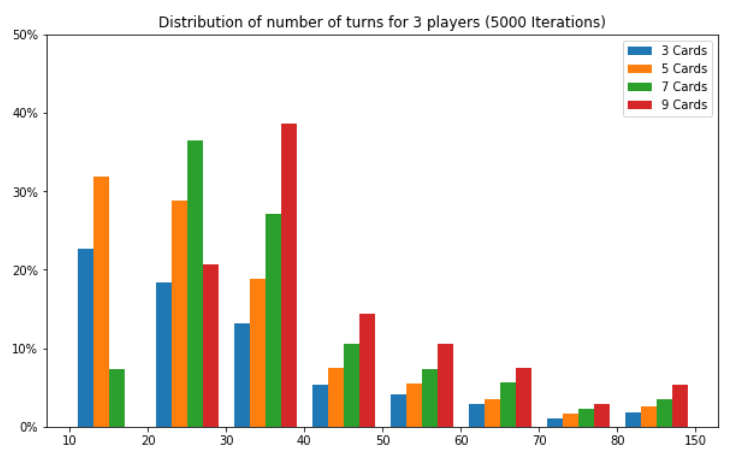
\includegraphics[width=0.9\textwidth]{histogram-cards}
\end{figure}


The histogram shows bars and percentage of games that end after 10-20 turns, 20-30 and so on. The more cards, the longer takes the game. The probability to finish after less than 20 turns is a bit to high with 3 or 5 cards in the beginning. 7 cards would mean that more than 50\% of the games would end after 20-40 turns.


Second analysis the impact of the number of players. I simulate Uno with 7 cards per player and 2-6 players per game. The histograms show the percentage of games that end with 10 to 20 turns, or 20 to 30 turns and so on. The last interval is from 80 to 150. You can see that most games end after 30-40 turns. And more player automatically leads to more turns, thats why I normalized the distribution by the number of players. Et voila, with 6 players it is very likely that the game ends in less than 20 rounds while with two players games can be very long. So 7 cards seems also be ok from this perspective, but maybe it’s worth to think about a 2-player version and name it Uno - Das Duell.


\begin{figure}[h!]
  \caption{\note{number of turns to finish the game}}
  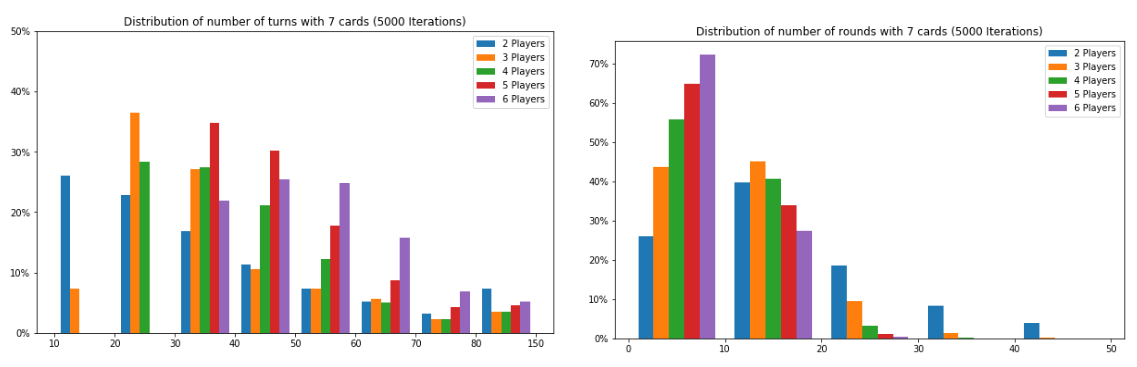
\includegraphics[width=0.9\textwidth]{histogram-players}
\end{figure}

\subsection{Verification and Validation}


One interesting question here is how often should I run the simulation. I observed the standard deviation every 100 iterations and it divergates after 5000

Last step is to analyze the result. 

Regargding Validation we can check for the three R’s.
(1) reality — how the model closely matches reality. The players in the game are simulated with a very simple and equal behavior. This won’t be the case in the real world. But the overall structure of the game exists.
(2) representation — some aspects are represented, some are not. I covered the basic concept but I decided to incorperate all special rules. This would increase the complexity but may not change the actual flow of the game.
(3) requirements — different levels of fi delity required for different applications. The requirement of the model was to answer the question of how many rounds does a game take and how could this be used for game balancing. This is also the reason why some aspects are not represented. E.g. thinking time or forget to say uno.


	%!TEX root=../report.tex

\section{Discussion}
	%!TEX root=../report.tex

\section{Conclusion}

This report introduces discrete-event simulations and classifies the purpose of discrete-event simulation based on its characteristics. Discrete-event simulations are stochastic, dynamic, and based on discrete events.
Every simulation is based on a model. A model can have a high or low fidelity, resolution, and scale. The introduced example of \uno\ has a low fidelity, low resolution, and high scale. A generic model of discrete-event simulation is the queuing of arriving events, followed by the processing of the events. Every event changes the system state. In the implementation of the card game framework, events are the turns of the individual players. The events occur at a fixed time. An event changes the system state. The evolution of the system state is logged. From these system states questions regarding the game evolution, can be answered. One shown example is the duration of \uno\ games. \uno\, which is played with seven hand cards, ends normally after 10-30 rounds. The simulation reveals that some special cards extend, some special cards shorten the game.
The implemented framework can be used to run a further analysis of \uno\ or other games as well. I can confirm discrete-event simulation can be used to simulate card games.

The Institute of Industrial Engineers published a list of advantages and disadvantages of simulations, that I would like to follow up on \cite{sokolowski2010modelingintro}. One advantage is that simulations enable us to make better decisions because every aspect can be tested. I can confirm this. I was able to look for games that take unexpectedly long and then visualize the game state to identify the bottleneck of the system.
Another advantage is to understand how a system operates. While implementing rules, I noticed how precise rules must be written down. So as a game developer I would always try to implement a simulation just to confirm that all aspects are covered.
But there are also disadvantages. Results need an interpretation. At some point, there is some uncertainty if the players are not implemented smart enough or if the game needs a modification.

All in all, discrete-event simulation is a powerful tool to reveal some hidden effects or to validate rules.



\newpage
% \bibliographystyle{chicago}
\bibliographystyle{plain}
\bibliography{bib}


\end{document}




% Questions:

% Code, Github. relevance?



% TODOS:


% add pages or chapters to citations

% introduction

% clean up github

